\chapter{Implementation Plan}
\section{Approach towards Software Development}
Features will be added to Issie using an incremental and Agile approach \cite{Voorhees2020}.
The incremental approach seeks to write code through a repeated cycle of three steps: (1) Analysis and Design, (2) Writing Code, and (3) Testing. A basic task/requirement is  broken into several parts - with each of these parts being written as an individual function \footnote{"individual function" does not refer to a single F\fsharp function, but to a top-level function which uses groups of helper and sub-functions}. Each function is tested both as a unit and when integrated into the codebase. All of these different parts build upon one another and come together to deliver the desired functionality. One caveat of the incremental approach is that the intermediate versions of the app are incomplete and therefore not suitable for any kind of release or proper demonstration. This can make it difficult to get proper feedback on the state of the application as a whole. This is acceptable within a short time-frame, but not for long-term software development over the course of the project. For that case, the Agile approach is considered. Small features, represented as a short sequence of stories, are built using the aforementioned incremental approach during sprints. Upon completion of this feature, it can be said that a new "product" (slightly improved version of Issie) has been delivered. During project meetings feedback can be obtained on the work completed, and any necessary adjustments will spawn new stories. Agile is generally used in continuous software development projects - and would be perfect for the long term development of Issie. However, due to the constraints of a Final Year Project: deadlines, need for planning and report writing, a pure Agile approach is not suitable. Instead, a hybrid approach will be pursued, which embodies Agile principles while still working within a plan-based framework. Provided that the backlog is intelligently structured, with tasks prioritised, and appropriate tolerances put in place such that project deadlines are met, such an approach is likely to yield success.

\section{Work completed as of the Interim Report deadline}

\subsection{Generating Truth Tables for a Sheet}
\emph{Associated Requirements:} \textbf{E1.1}, \textbf{E1.3}, \textbf{E1.6}

The first task undertaken was to generate a standard truth table for a sheet in Issie containing only combinational logic. Given that Issie already features a performant and reliable simulator (step simulator) for calculating the outputs combinational logic, the decision was made to use as much of its implementation as possible. This approach has many advantages:
\begin{itemize}
    \item The existing step simulator has been extensively tested by end-users, meaning that its implementation is most likely bug-free. By using it, it will reduce the chance of the new feature introducing new bugs.
    \item In most cases, reusing existing code is much faster than writing new code from scratch. Not only is time saved on writing new code, but the amount of time spent debugging is also reduced.
    \item Reusing existing code will help keep the overall size of the codebase small. Not only does this help future programmers who work on the project by reducing how much they have to understand, but it also means that any future performance improvements made to the simulation code are also improvements to Truth Table generation.
\end{itemize}

Figure \ref{fig:flowchartSim} provides an overview of Issie's process for building and running a Step Simulation. In this process, various checks must be performed; firstly the logic designed by the user must be verified to be syntactically correct, secondly the organisation of project files must be correct, and thirdly some Issie specific limitations (e.g. no cycles in combinational logic) must be enforced. Issie's simulation building process can be said to have three levels, with each level having an associated data structure which represents schematic. These data structures are: the \textbf{Canvas State}, \textbf{Simulation Data/Error}, and a \textbf{Fast Simulation}. A set of checks are performed at each level, and only upon passing these checks can a schematic be transformed to the subsequent data structure.
If any of these checks fail due to an issue with the user's schematic, the simulation building process returns a \textit{SimulationError}, which tells the user what the error is and which components/connections are affected. A key takeaway from Figure \ref{fig:flowchartSim} is that the process of building a simulation is separate to the process of running it. Any changes made to the values of inputs and outputs are fed directly into the Fast Simulation. The truth table generation functionality makes use of this property.

Truth Table generation for a whole sheet can be broken down into the following stages:
\begin{enumerate}
    \item Build Simulation Data using the same methods as the Step simulator.
    \item Ensure that all logic is combinational.
    \item Get all Simulation Inputs and Outputs from the Simulation Data.
    \item Calculate the Left-hand side of the Truth Table by finding all combinations of input values.
    \item For each input combination:
    \begin{enumerate}
        \item Feed input combination into the Fast Simulation.
        \item Extract outputs from the Fast Simulation.
        \item Record the input/output mapping in the Truth Table structure.
    \end{enumerate}
    \item Visualise the Truth Table
\end{enumerate}

%%%%% Commands (variables) for type information %%%%%
% Cell Table Data
\newcommand{\ttCellData}{
    Discriminated Union type representing what data each truth table cell can hold. Cells can hold Bits (represented by Issie's WireData type), Algebraic expressions (represented by strings), or a Don't Care.
}

% TT Cell
\newcommand{\ttCell}{
    Record type which represents the contents of a cell in a truth table. Contains Cell Data and a Simulation IO (the input or output that the data corresponds to).
}

% TT Row
\newcommand{\ttRow}{
    Represents a row in a truth table, which is a list of Truth Table Cells.
}

% TT
\newcommand{\truthtable}{
    Record type containing a Map data structure which maps a row of inputs to a row of outputs, as well as other information about the truth table (scope of of this TBD).
}

\subsubsection{Data Type Hierarchy for Truth Tables}
\begin{table} [h!]
    \centering
    \begin{tabular}{| m{4cm} | m{10cm} |}
        \hline
        \textbf{Data Type/Structure} & \textbf{Information} \\
        \hline
        Cell Data & \ttCellData \\
        \hline
        Truth Table Cell & \ttCell \\
        \hline
        Truth Table Row & \ttRow \\
        \hline
        Truth Table & \truthtable \\
        \hline
    \end{tabular}
\end{table}

\subsubsection{Calculating LHS Combinations for 1-bit inputs}
A truth table with $n$ inputs will have $2^n$ rows. For example, the truth table for a multiplexer (Table \ref{subfig:muxTT_standard}) shown in Section \ref{subsec:TruthTables} has three inputs and eight rows. All input rows can be calculated by counting from $0$ to $2^n-1$ in binary with an $n$-bit representation. This is seen in Table \ref{subfig:muxTT_standard}, with the first row corresponding to 0 (0 | 0 | 0), and the last row corresponding to 7 (1 | 1 | 1).

\subsubsection{General Algorithm for Calculating LHS Combinations}
While the basic method of turning a sequence of binary numbers into rows works for 1-bit inputs, this is not sufficient for Issie, which lets users have buses as inputs (multi-bit inputs). There were two possible approaches for handling input buses. The easier approach implementation-wise would have involved simply treating each bit of the bus as an individual 1-bit input and using the 1-bit input logic for calculating combinations. However, this is not user-friendly at all - for example a 32 bit bus would be split into 32 different inputs. This would massively increase the number of columns in the truth table, impacting the utility of the truth table as an aid. Instead, the decision was made to represent each multi-bit input/output as one column in the truth table, with a hexadecimal value. 
The algorithm first separates 1-bit inputs from multi-bit inputs, then calculates and stores all combinations of those inputs. Combinations of multi-bit inputs with each another are then handled separately. If a given input has a width of $n$ bits, it can take a total of $2^n$ values. If there are $k$ multi-width inputs, and if we define a set $S_i$ as the set of all possible input combinations for the $i$th multi-bit input, then the set of all possible input combinations is:
\begin{equation}
    \prod_{i=1}^{k} S_i
\end{equation}
Where $\prod$ represents the \textbf{Cartesian} product of sets. For only two multi-bit inputs, the library function \codestyle{List.allPairs} \cite{ListFuns} can be used to find this Cartesian product, with each set of possible values being passed in as a List. However, no such library function exists for $k$ sets/lists. The function \codestyle{numbComb} was implemented to find the Cartesian product of $k$ lists. The function is tail recursive for improved performance.

\subsubsection{Visualising Truth Tables}
As of the Interim report, Truth Tables are visualised using Fulma Tables. They are clear, responsive and do a good job overall. However, they lack interactivity. Therefore, it is anticipated that they will be replaced or modified in the future. For viewing multi-bit inputs and outputs, hexadecimal was chosen over binary as it would take up less physical space. Currently, there is no option to change number base (as there is in the Step Simulator), but this would be trivial to implement in the future. Truth Table generation and viewing is done in an MVU way; pressing the "Generate Truth Table" button causes a truth table to be generated and stored in the \textbf{Model} through a message which is processed by the \textbf{Update} function. On the next call of the View function, this Truth Table is rendered.


\begin{figure} [h!]
    \centering
    \includegraphics[width=\textwidth]{04.ImpPlan/IssieSim.png}
    \caption{An overview of Issie's Step Simulation}
    \label{fig:flowchartSim}
\end{figure}

\newpage % Here to ensure flowchart figure is in the right place

\subsection{Generating Truth Tables for a partial selection of a Sheet}
\emph{Associated Requirements:} \textbf{E1.2}, \textbf{E1.3}

The motivation behind Requirement \textbf{E1.2} is that a large schematic with lots of components will often contain smaller blocks of logic within it. These blocks may be defined Custom Components, or simply be a collection of gates in one corner of the canvas. Either way, there is value in the user being able to isolate these blocks and learn about the combinational logic implemented by them. Such functionality would also allow users to take a divide-and-conquer approach to debugging logical errors - individual blocks could be inspected to ascertain if they had been implemented correctly. 

A challenge with generating a truth table from part of a canvas is that Issie has no existing method for simulating part of a canvas. When working with a whole sheet, the inputs and outputs are well-defined; sheets where any ports aren't connected to inputs/outputs throw \textit{Simulation Errors}. In contrast, a partial selection from a sheet will rarely contain all inputs and outputs. Two methods were considered for simulating the selected logic to generate a truth table, with the latter being chosen.
\begin{enumerate}
    \item \textbf{Extracting the Fast Simulation and feeding values into specific wires}. This method would have involved creating a Fast Simulation for the whole sheet as usual, but then manually changing values in component arrays and seeing how those changes propagated through to the output connections of the selected logic. While this method seemed fit initially, several issues were found after some analysis. The Fast Simulation would be built for the whole sheet, meaning that an error elsewhere on the canvas would stop the selected logic from being simulated. Custom Components would also be harder to manage as the Fast Simulation datatype flattens the design, meaning that all nested logic in Custom Components would be expanded out. The new logic would also be quite different from the truth table generation logic for whole sheets - this is not ideal for future code maintenance purposes.
    \item \textbf{Intelligently building and correcting a new Canvas}. Following the highlighting of the issues with the first approach, an alternative approach was put forward. Rather than attempting to work with the complicated Fast Simulation data structure, it instead aims to use as much of the existing code as possible by treating the selected logic as a separate instance of a Canvas State and trying to simulate it using the same method as simulating a whole canvas. The main difference between simulating a whole sheet and simulating selected logic is the lack of guaranteed input and output components. This is overcome by finding which ports/connections are inputs/outputs for the selected logic, then intelligently adding 'phantom' input/output components to the canvas in a process called Canvas Correction. Once a corrected canvas corresponding to the selected logic is created, the logic used for generating and viewing a Truth Table for a whole sheet can be reused.
\end{enumerate}

Prior to the canvas correction stage, the selected components are checked. If only connections are selected, then a \textit{Simulation Error} is returned to the user informing them of their mistake.

\subsubsection{Canvas Correction}
\begin{itemize}
    \item[Step 1] \textbf{Add Extra Connections:} Sub-figures \ref{subfig:SelCase2} to \ref{subfig:SelCase4} in Figure \ref{fig:SelCases} all show situations where one or more inputs/outputs for the selected logic are ports on components, rather than connections. Taking the case shown in Figure \ref{subfig:SelCase2} in particular, the inputs to the selected logic are: both input ports on G1, and the bottom input port on G2, while the outputs from the selected logic are both output ports on G1 and G2 respectively. Prior to correction, the selection canvas does not have any connections going into those ports. This step finds any ports on selected components which do not have a connection in the selection and connects them to "dummy" input or output ports depending on their \codestyle{PortType}. This transforms the canvas to a state similar to that seen in Case (a), where   all inputs into the selected logic have connections.
    \item[Step 2] \textbf{Add Extra IOs:} This step adds the "phantom" input and output components to the selection canvas. The locations where these components need to be inserted are found by checking which connections in the Canvas State do not have both ports present in the selection. Any such connections are either connected to some other component in the sheet which is not selected, or are newly added connections which are connected to dummy ports. Either way, these are the connections that need to be connected to "phantom" IOs. 
    \begin{itemize}
        \item[Step 2.1] \textbf{IO Width Inference:} When creating new input or output components, the correct width must be specified. This is         calculated by running Issie's \codestyle{WidthInferrer} on the whole sheet to find the expected width of the input or output. However, in cases such as the one shown in Figure \ref{subfig:SelCase4}, where there are no connections to/from some ports on G3, \codestyle{WidthInferrer} will fail to infer widths, resulting in a \textit{Simulation Error}. A possible workaround would be to try to infer the width from the component itself if \codestyle{WidthInferrer} fails - in Issie AND gates always have 1-bit inputs, so any "phantom" inputs generated would have a width of one. This would be trivial to implement in the future. However, there would still be cases, such as inputs into multiplexers and n-bit XORs, where even this approach would not work.
        \item[Step 2.2] \textbf{IO Label Inference:} Usually users provide labels for IOs, which are used in the Truth Table. However, when IOs are automatically created, names for them must be automatically generated too. This is done by looking at which ports in the selection they are connected to. The expression for an automatically generated IO Label is: \codestyle{[Connected Component Label]\_[IN/OUT][SUFFIX]}. If the port is labelled (e.g. on a multiplexer or a Custom Component), the suffix is the port label. Alternatively it is the \codestyle{PortNumber}, which indicates the position of a port on its host component.
        
    \end{itemize} 
    \item[Step 3] \textbf{Returning a Canvas or an Error:} If any errors were found in the previous steps, most likely due to a malformed selection, they are returned. If not, then the returned Canvas State is completely compatible with the existing simulation and truth table generation functions.
\end{itemize}

Following Canvas Correction, any returned Canvas State is fully compatible with the existing functions for simulating logic and generating truth tables. Therefore, a Truth Table can be generated for selected logic through the same methods and functions used for generating Truth Tables for the whole sheet.

\bigskip
\begin{figure} [h]
    \begin{subfigure}{0.48\textwidth}
        \centering
        \includegraphics[width=0.8\linewidth]{04.ImpPlan/SelCase1.png}
        \caption{Case where all inputs into selected logic are connections.}
        \label{subfig:SelCase1}
    \end{subfigure}
    \begin{subfigure}{0.48\textwidth}
        \centering
        \includegraphics[width=0.8\linewidth]{04.ImpPlan/SelCase2.png}
        \caption{Case where some inputs into selected logic are connections, and some are ports on components.}
        \label{subfig:SelCase2}
    \end{subfigure}
    \newline
    \begin{subfigure}{0.48\textwidth}
        \centering
        \includegraphics[width=0.8\linewidth]{04.ImpPlan/SelCase3.png}
        \caption{Case where selected logic includes an input component.}
        \label{subfig:SelCase3}
    \end{subfigure}
    \begin{subfigure}{0.48\textwidth}
        \centering
        \includegraphics[width=0.8\linewidth]{04.ImpPlan/SelCase4.png}
        \caption{Case where a selected component does not have connections to all ports}
        \label{subfig:SelCase4}
    \end{subfigure}
    \caption{Selection Cases}
    \label{fig:SelCases}
\end{figure}

\subsection{UI Changes}
\emph{Associated Requirements:} \textbf{D3.1}
As mentioned in Section \ref{sec:IssieUI}, there are inconsistencies in Issie's current UI, particularly concerning the Waveform Simulator. With the addition of Truth Table viewing to Issie, the decision was made to tweak the UI to try to keep everything consistent. Figures \ref{fig:OldUI} and \ref{fig:NewUI} show the old and newly tweaked UIs respectively. The top bar primarily houses operations or information concerning files, such as the button to save the sheet, menu to open other sheets/projects, and the filepath. As a result the \textit{Waveforms} button has been removed from there. Ideally it would have a permanent place on the right tab, however with the addition of a Truth Table tab this would take the total number of tabs up to five, causing the tab label text to become illegible.  Given that there are now three ways to gain an insight into the logic on the sheet (Step Simulator, Truth Tables, Waveform Simulator), it is logical to group these together as sub-tabs under one main tab. The new UI now always has three tabs on the right in contrast to the old UI which would spawn the WaveSim tab when viewing Waveforms. Clicking the right-most "Simulations" tab will now reveal three sub-tabs: Step Simulation, Truth Tables, and Wave Simulation. The behaviour of the Truth Table view and the updated WaveSim view is modelled on that of the Step Simulator. Selecting a tab for the respective simulator will reveal a short description of the function, and a button to start the appropriate action. The colour and message shown by this button is dependent on the sheet: problems will show a yellow button, and a solid green button shows that the sheet is correct, and the functionality is available. Light green means that while the sheet is syntactically correct, some other factor is making the functionality unavailable. For the Waveform simulator this is when the sheet contains no synchronous logic (meaning no waveforms to display), and for Truth Tables it is when the sheet does contain synchronous logic (as synchronous logic is currently not supported for truth tables).

\begin{figure}
    \centering
    \includegraphics[width=0.8\textwidth]{04.ImpPlan/OldUI.png}
    \caption{Old Issie UI}
    \label{fig:OldUI}
\end{figure}

\begin{figure}
    \centering
    \includegraphics[width=0.8\textwidth]{04.ImpPlan/NewUI.png}
    \caption{New Issie UI}
    \label{fig:NewUI}
\end{figure}

\section{Work Breakdown Structure}
As with any large project, a key stage in planning is to break it down into several manageable chunks. This has been done to some extent in the Requirements Capture (Chapter \ref{chap:requirements}), albeit at quite a high level. On the other hand, a Work Breakdown Structure (WBS) \cite{projectmanagement} defines the scope of the project and breaks the work down into components that can be scheduled, monitored, and controlled. This aids in assessing the complexity of certain tasks, therefore improving the overall distribution of resources (mainly time) to different tasks. The WBS for this project is shown in Figure \ref{fig:wbs} - it is rotated to make it more clear to the viewer. Red nodes in the WBS could be considered as \emph{Initiatives}, as they are long term (relative to the length of the project) objectives. Green nodes are rough equivalents to \emph{Epics}, and white/grey nodes are \emph{User Stories}. In some cases, user stories may have very short sub-tasks underneath them which need not necessarily be differentiated, but are done on the WBS for clarity's sake. User Stories which spawn sub-tasks are coloured purple, while sub-tasks requiring further elaboration are coloured yellow. 

\section{Time Management and Gantt Chart}
Effective time management is vital to any project; traditionally a Gantt chart is used to display the timeframe in which the tasks detailed in the WBS will be completed. In line with this, a Gantt chart has been prepared for this project, and can be seen in Figure \ref{fig:gantt}. The colour coding on the chart matches that on the WBS, and key deadlines are indicated by dashed vertical lines. The first line represents the Interim report deadline - therefore any work shown on the chart to the left of this line is already completed, while any work to the right of the line is planned. The layout of Figure \ref{fig:gantt} allows it to double as a chronologically structured backlog. Within Initiatives, Epics are placed in chronological order, and likewise for User Stories within Epics. Two main considerations were made when devising this order of items. Firstly, dependencies were considered - for example it would be foolish to write code to view truth tables prior to there being a mechanism to generate them. Secondly, the importance of the deliverable associated with a task was taken into account - with tasks that fulfilled essential requirements given precedence over those that fulfilled desired requirements. 

\subsection{Contingencies and Strategies taken to Mitigate Risk}
The project plan has been structured to contain a healthy contingency allowance. Looking at the order of work in the Gantt chart, it can be seen that all essential requirements (and the majority of the desired features) should be fulfilled by the beginning of May. Furthermore, all technical work is expected to be completed by the end of May, bar a possible need to reconfigure parts of Issie's overall GUI (which is very unlikely).
Additionally, most time estimations for tasks have some margin built in as well, reducing the likelihood of technical work overrunning. This leaves the last three weeks of the project dedicated solely to report writing and documentation; two tasks which ideally will have been worked on over the duration of the project. Therefore, this plan yields a contingency allowance of three weeks.
The project management strategy, formed by a fusion of plan-based and Agile management methods, also acts as a form of contingency. As stated, the backlog ordering methodology has taken into account dependencies and importance of deliverables. If progress is slow, then the backlog can be dynamically reorganised, with less essential items shifted or removed. The ultimate fallback is to only implement the essential features, but such an extreme case is highly unlikely to arise. On the other hand, if progress runs ahead of schedule extension tasks can be discussed.

\begin{figure}
    \centering
    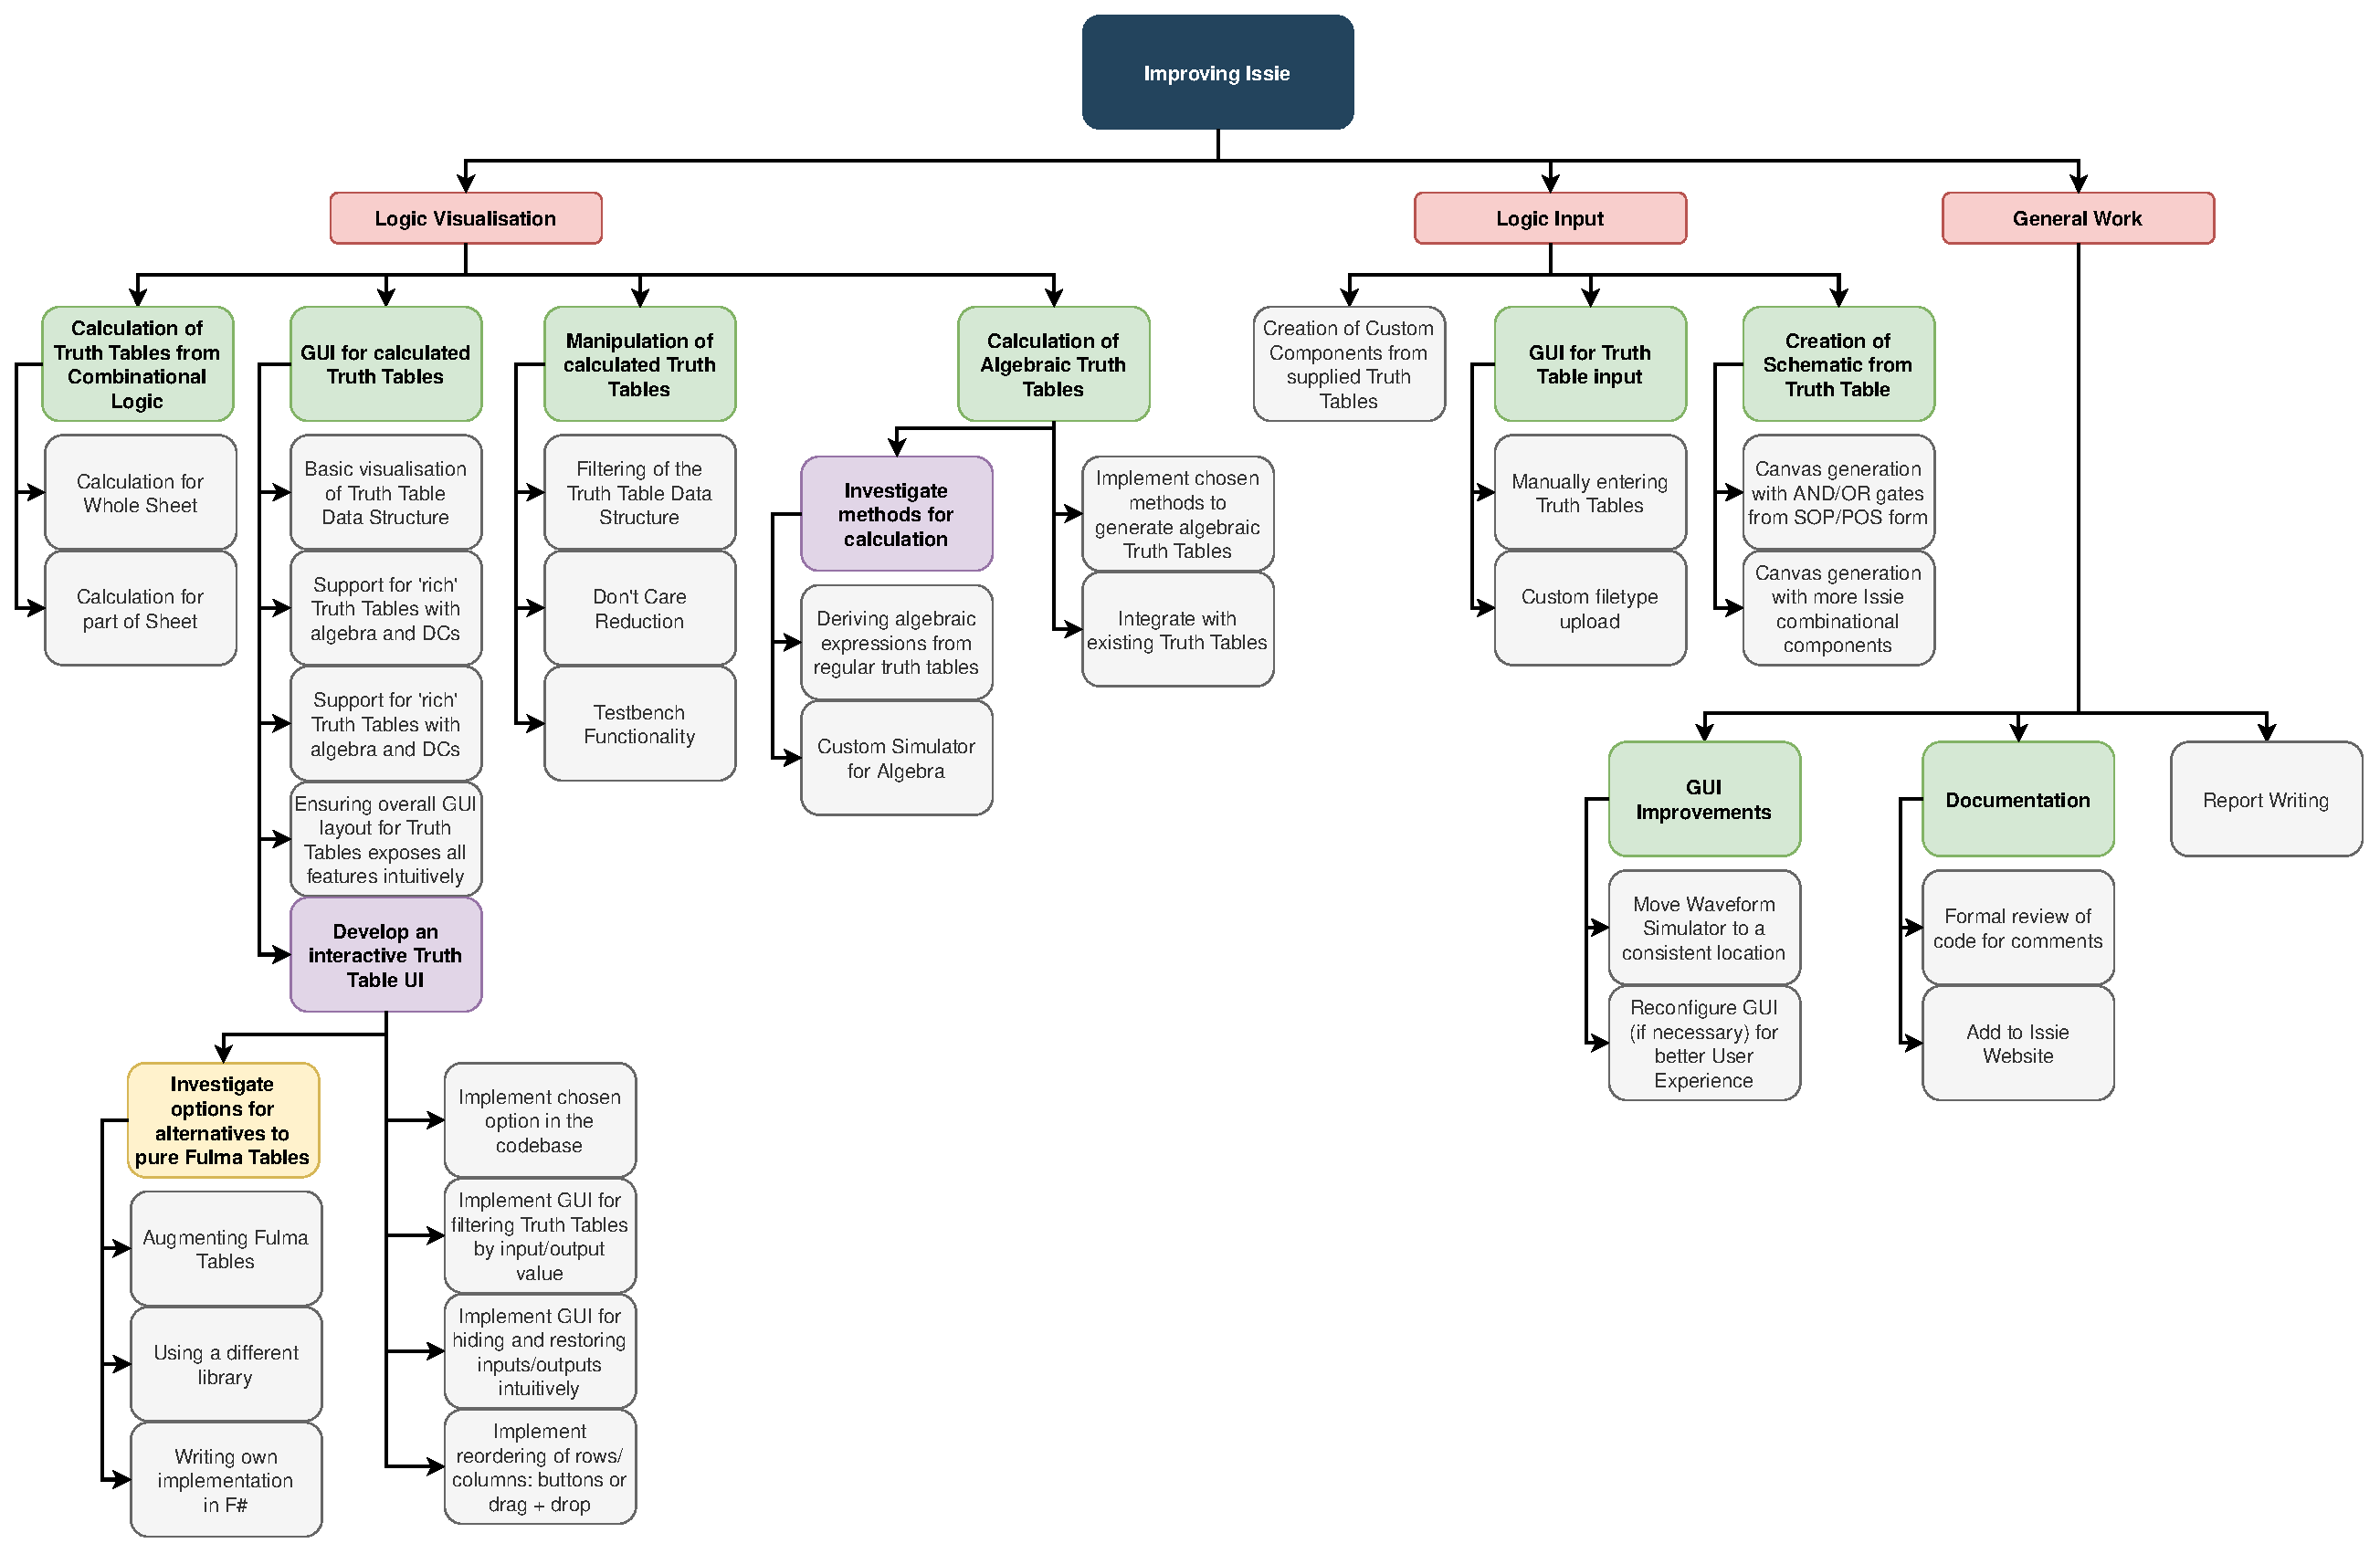
\includegraphics[width=22cm,angle=270,origin=c]{04.ImpPlan/wbs.eps}
    \caption{Work Breakdown Structure for the Project (Rotated)}
    \label{fig:wbs}
\end{figure}

\begin{figure}
    \centering
    \includegraphics*[width=\textwidth]{04.ImpPlan/gantt_update.pdf}
    \caption{Gantt Chart for the Project}
    \label{fig:gantt}
\end{figure}